\section{The uncertain Darcy problem}
The two methods for approximating the mean exit time have been investigated in a general frame. In the following we will consider \eqref{eq:GeneralModel} with $f\colon \mathbb{R}^2 \rightarrow \mathbb{R}^2$ given by the solution of the uncertain Darcy problem. 

\subsection{Problem statement}
Let us consider a domain $D \subset \mathbb{R}^2$. Let us define the Neumann boundaries of $D$ as $\Gamma_N$, its inlet boundary as $\Gamma_{in}$ and its outlet boundary as $\Gamma_{out}$. Then, we search the solution of the following problem
\begin{equation}
	\label{eq:DarcyProblem}
	\left \{
  	\begin{aligned}
		u &= -A \nabla p, && \text{in } D, \\
		\nabla\cdot u &= 0, && \text{in } D, \\
		p &= p_0, && \text{on } \Gamma_{in},\\
		p &= 0, && \text{on } \Gamma_{out}, \\
		\nabla p &= 0, && \text{on } \Gamma_N,
	\end{aligned} \right.
\end{equation}
where $A$ is a random field. The solution $u$ of this equation is used as transport field in equation \eqref{eq:GeneralModel}, which can be therefore written as
\begin{equation}\label{eq:GeneralDarcySDE}
  	\left \{
  	\begin{aligned}
    		dX(t) &= u(X) dt + \sigma dW(t), && 0 < t \leq T, \\
    		X(0)  &= X_0, 	 	     && X_0 \in D,
  	\end{aligned} \right.
\end{equation} 

where we set the boundary conditions to be reflecting on $\Gamma_N$ and killing on both $\Gamma_{in},\Gamma_{out}$.

\begin{figure}[t]
    \centering
    \begin{subfigure}{0.49\linewidth}
        \centering
        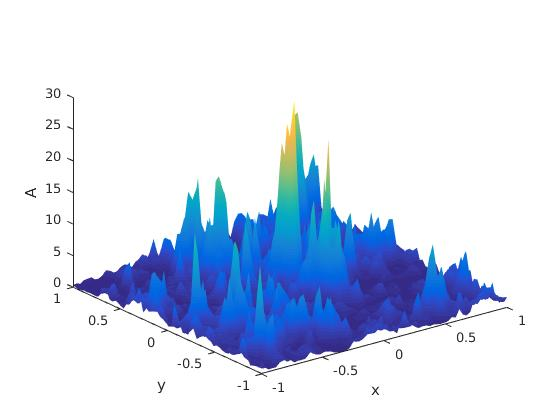
\includegraphics [width=1\linewidth]{Darcy/Pictures/A.jpg}
        \caption{Random field.}
        \label{fig:DarcyA}
    \end{subfigure}
    \begin{subfigure}{0.49\linewidth}
        \centering
        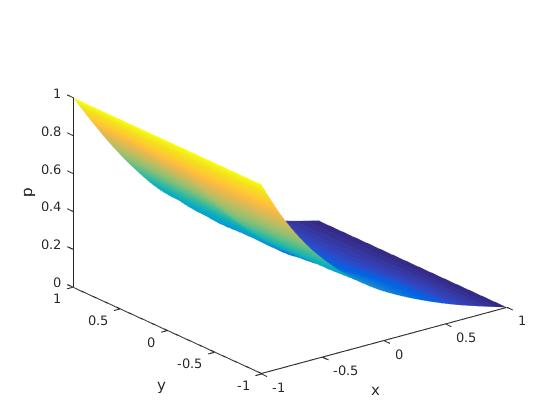
\includegraphics [width=1\linewidth]{Darcy/Pictures/P.jpg}
        \caption{Pressure field.}
        \label{fig:DarcyP}
    \end{subfigure}    
    \begin{subfigure}{0.49\linewidth}
        \centering
        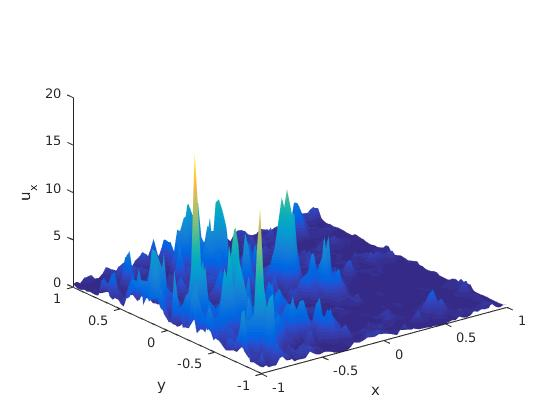
\includegraphics [width=1\linewidth]{Darcy/Pictures/Ux.jpg}
        \caption{$x$ component of velocity field.}
        \label{fig:DarcyUx}
    \end{subfigure}
    \begin{subfigure}{0.49\linewidth}
        \centering
        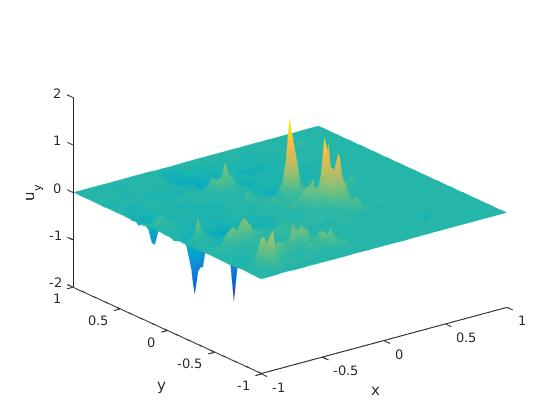
\includegraphics [width=1\linewidth]{Darcy/Pictures/Uy.jpg}
        \caption{$y$ component of velocity field.}
        \label{fig:DarcyUy}
    \end{subfigure}    
    \caption{Approximate solution of the uncertain Darcy problem.}
    \label{fig:DarcyResults}
\end{figure}



\subsection{Finite Elements solution of the Darcy problem}

Let us consider the domain $D = [-1,1] \times [-1,1]$. The random field $A$ in \eqref{eq:DarcyProblem} is chosen to be lognormal, \textit{i.e.}, 
\begin{equation}\label{eq:RandomField}
	A = e^\gamma,
\end{equation}
where $\gamma$ is a normal random field defined by its covariance function $\mathrm{cov}_\gamma(x_1,x_2)$ for any couple of points $x_1,x_2$ in the domain $D$. The covariance function is of the Matern family, thus having the following form
\begin{equation}\label{eq:CovFunction}
	\mathrm{cov}_\gamma(x_1,x_2) = \frac{\sigma^2}{\Gamma(\nu)2^{\nu-1}}\Big(\sqrt{2\nu}\frac{|x_1-x_2|}{L_c}\Big)^\nu K_{\nu}\Big(\sqrt{2\nu}\frac{|x_1-x_2|}{L_c}\Big), \quad \nu \geq 0.5,
\end{equation}
where $\sigma^2$ is the variance, $L_c$ is the correlation length, $\Gamma$ is the gamma function, $K_\nu$ is the modified Bessel function of the second kind and $\nu$ is a parameter. Let us remark that the covariance function does not depend on $x_1, x_2$ but only on their euclidean distance $|x_1 - x_2|$. The regularity of the covariance function and of the realizations of $A$ depend on $\nu$. In particular, for $\nu$ equal to 0.5, the covariance is Lipschitz continuous and the field is $\alpha$-Hölder continuous for $\alpha < 0.5$. Results concerning regularity properties of $A$ can be found in \cite{Nobile2015}. The realizations of $A$ are computed using a discrete Fourier transformation on the vertices of a grid of $D$, equispaced on both the $x$ and $y$ directions with the same spacing $\Delta_A$. Then, the numerical solution $p_h$ of \eqref{eq:DarcyProblem} is obtained with linear Finite Elements on a regular mesh $T_p$ with maximum element size $\Delta_p$. Since the vertices of the grid on which we compute $A$ do not coincide with the vertices of $T_p$, we interpolate $A$ on $T_p$ to obtain $p_h$. Then, the velocity field $u_h$ is retrived computing the gradient on $p_h$. The results for a realization of $A$ are shown in Figure \ref{fig:DarcyResults}, where the value of the inlet pressure $p_0$ is equal to 1, and the parameters for the random field are $\nu = 0.5, L_c = 0.05$. 


\subsection{Solution of the SDE}

Once the Finite Element approximation $u_h$ of the velocity field is available, it is possible to approximate by means of DEM and CEM the solution of \eqref{eq:GeneralDarcySDE}. The values of the numerical solution $X_h$ can take any value in $D$, therefore it is necessary that the velocity field is defined in any point in $D$. If an interpolation of $u_h$ is performed at each step, both DEM and CEM lose in computational efficiency. Hence, an interpolation of $u_h$ has to be performed before the numerical integration of the SDE. We choose to exploit the grid defined by $\Delta_A$, interpolating the values of $u_h$ in the center of each square (Figure \ref{fig:GridVelocity}). Let us denote by $Q$ the set of the interpolation points, whose elements are defined by
\begin{equation}\label{eq:InterpMatrix}
	\{Q\}_{ij} = \begin{pmatrix} -1 + (i-0.5)\Delta_A, & -1 + (j-0.5)\Delta_A \end{pmatrix}^T, \quad i,j = 1, \dots, \frac{2}{\Delta_A} =: N_A.
\end{equation}
We compute two matrices $U_x, U_y$ of $\mathbb{R}^{N_A \times N_A}$ containing the values of the two components of $u_h$ interpolated on the points of $Q$. Then, the velocity field is considered to be piecewise constant in each square of the grid defined by $\Delta_A$. Therefore, if we denote by $\tilde{u}$ the transport field for the SDE, at the $i$-th step of the integration $\tilde{u}$ is evaluated as follows
\begin{equation}\label{eq:VelEval}
	\tilde{u}(X_h(t_i)) = \begin{pmatrix}	U_x(\ceil{(X_{h,1}(t_i)+1)/\Delta_A},\ceil{(X_{h,2}(t_i)+1)/\Delta_A}) \\
					U_y(\ceil{(X_{h,1}(t_i)+1)/\Delta_A},\ceil{(X_{h,2}(t_i)+1)/\Delta_A}) \end{pmatrix},
\end{equation}
where $X_{h,1}, X_{h,2}$ denote the first and second components of $X_h$ and $U_x(i,j)$ represents the element $(i,j)$ of the matrix $U_x$ (respectively $U_y$). Then, given the step size $h$, one step of DEM will be defined as
\begin{equation}\label{eq:DEMDarcy}
	X_h(t_{i+1}) = \tilde{u}(X_h(t_i)) h + \sigma (W(t_{i+1}) - W(t_i)).
\end{equation}

\begin{figure}[t]
    \centering
    \resizebox{0.8\linewidth}{!}{% This file was created by matlab2tikz.
%
%The latest updates can be retrieved from
%  http://www.mathworks.com/matlabcentral/fileexchange/22022-matlab2tikz-matlab2tikz
%where you can also make suggestions and rate matlab2tikz.
%
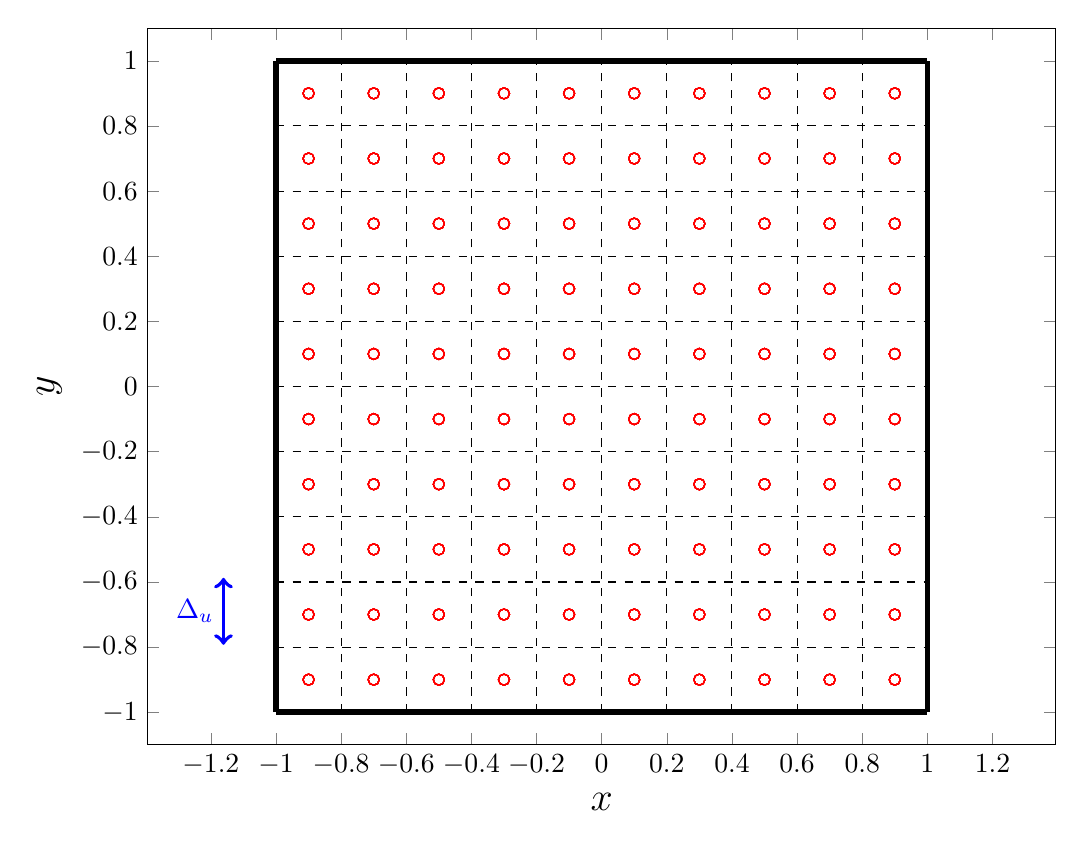
\begin{tikzpicture}



\begin{axis}[%
width=4.542in,
height=3.583in,
at={(0.801in,0.484in)},
scale only axis,
xmin=-1.39468302658487,
xmax=1.39468302658487,
xlabel={$x$},
xlabel style={font=\Large},
ymin=-1.1,
ymax=1.1,
ylabel={$y$},
ylabel style={font=\Large},
axis background/.style={fill=white}
]
\addplot [color=black,solid,line width=2.0pt,forget plot]
  table[row sep=crcr]{%
-1	-1\\
-1	1\\
};
\addplot [color=black,solid,line width=2.0pt,forget plot]
  table[row sep=crcr]{%
1	-1\\
1	1\\
};
\addplot [color=black,solid,line width=2.0pt,forget plot]
  table[row sep=crcr]{%
-1	-1\\
1	-1\\
};
\addplot [color=black,solid,line width=2.0pt,forget plot]
  table[row sep=crcr]{%
-1	1\\
1	1\\
};
\addplot [color=black,dashed,forget plot]
  table[row sep=crcr]{%
-1	-0.8\\
1	-0.8\\
};
\addplot [color=black,dashed,forget plot]
  table[row sep=crcr]{%
-0.8	-1\\
-0.8	1\\
};
\addplot [color=red,only marks,mark=o,mark options={solid},forget plot]
  table[row sep=crcr]{%
-0.9	-0.9\\
-0.9	-0.7\\
-0.9	-0.5\\
-0.9	-0.3\\
-0.9	-0.1\\
-0.9	0.1\\
-0.9	0.3\\
-0.9	0.5\\
-0.9	0.7\\
-0.9	0.9\\
};
\addplot [color=red,only marks,mark=o,mark options={solid},forget plot]
  table[row sep=crcr]{%
-0.9	-0.9\\
-0.9	-0.7\\
-0.9	-0.5\\
-0.9	-0.3\\
-0.9	-0.1\\
-0.9	0.1\\
-0.9	0.3\\
-0.9	0.5\\
-0.9	0.7\\
-0.9	0.9\\
};
\addplot [color=red,only marks,mark=o,mark options={solid},forget plot]
  table[row sep=crcr]{%
-0.9	-0.9\\
-0.9	-0.7\\
-0.9	-0.5\\
-0.9	-0.3\\
-0.9	-0.1\\
-0.9	0.1\\
-0.9	0.3\\
-0.9	0.5\\
-0.9	0.7\\
-0.9	0.9\\
};
\addplot [color=red,only marks,mark=o,mark options={solid},forget plot]
  table[row sep=crcr]{%
-0.9	-0.9\\
-0.9	-0.7\\
-0.9	-0.5\\
-0.9	-0.3\\
-0.9	-0.1\\
-0.9	0.1\\
-0.9	0.3\\
-0.9	0.5\\
-0.9	0.7\\
-0.9	0.9\\
};
\addplot [color=red,only marks,mark=o,mark options={solid},forget plot]
  table[row sep=crcr]{%
-0.9	-0.9\\
-0.9	-0.7\\
-0.9	-0.5\\
-0.9	-0.3\\
-0.9	-0.1\\
-0.9	0.1\\
-0.9	0.3\\
-0.9	0.5\\
-0.9	0.7\\
-0.9	0.9\\
};
\addplot [color=red,only marks,mark=o,mark options={solid},forget plot]
  table[row sep=crcr]{%
-0.9	-0.9\\
-0.9	-0.7\\
-0.9	-0.5\\
-0.9	-0.3\\
-0.9	-0.1\\
-0.9	0.1\\
-0.9	0.3\\
-0.9	0.5\\
-0.9	0.7\\
-0.9	0.9\\
};
\addplot [color=red,only marks,mark=o,mark options={solid},forget plot]
  table[row sep=crcr]{%
-0.9	-0.9\\
-0.9	-0.7\\
-0.9	-0.5\\
-0.9	-0.3\\
-0.9	-0.1\\
-0.9	0.1\\
-0.9	0.3\\
-0.9	0.5\\
-0.9	0.7\\
-0.9	0.9\\
};
\addplot [color=red,only marks,mark=o,mark options={solid},forget plot]
  table[row sep=crcr]{%
-0.9	-0.9\\
-0.9	-0.7\\
-0.9	-0.5\\
-0.9	-0.3\\
-0.9	-0.1\\
-0.9	0.1\\
-0.9	0.3\\
-0.9	0.5\\
-0.9	0.7\\
-0.9	0.9\\
};
\addplot [color=red,only marks,mark=o,mark options={solid},forget plot]
  table[row sep=crcr]{%
-0.9	-0.9\\
-0.9	-0.7\\
-0.9	-0.5\\
-0.9	-0.3\\
-0.9	-0.1\\
-0.9	0.1\\
-0.9	0.3\\
-0.9	0.5\\
-0.9	0.7\\
-0.9	0.9\\
};
\addplot [color=red,only marks,mark=o,mark options={solid},forget plot]
  table[row sep=crcr]{%
-0.9	-0.9\\
-0.9	-0.7\\
-0.9	-0.5\\
-0.9	-0.3\\
-0.9	-0.1\\
-0.9	0.1\\
-0.9	0.3\\
-0.9	0.5\\
-0.9	0.7\\
-0.9	0.9\\
};
\addplot [color=black,dashed,forget plot]
  table[row sep=crcr]{%
-1	-0.6\\
1	-0.6\\
};
\addplot [color=black,dashed,forget plot]
  table[row sep=crcr]{%
-0.6	-1\\
-0.6	1\\
};
\addplot [color=red,only marks,mark=o,mark options={solid},forget plot]
  table[row sep=crcr]{%
-0.7	-0.9\\
-0.7	-0.7\\
-0.7	-0.5\\
-0.7	-0.3\\
-0.7	-0.1\\
-0.7	0.1\\
-0.7	0.3\\
-0.7	0.5\\
-0.7	0.7\\
-0.7	0.9\\
};
\addplot [color=red,only marks,mark=o,mark options={solid},forget plot]
  table[row sep=crcr]{%
-0.7	-0.9\\
-0.7	-0.7\\
-0.7	-0.5\\
-0.7	-0.3\\
-0.7	-0.1\\
-0.7	0.1\\
-0.7	0.3\\
-0.7	0.5\\
-0.7	0.7\\
-0.7	0.9\\
};
\addplot [color=red,only marks,mark=o,mark options={solid},forget plot]
  table[row sep=crcr]{%
-0.7	-0.9\\
-0.7	-0.7\\
-0.7	-0.5\\
-0.7	-0.3\\
-0.7	-0.1\\
-0.7	0.1\\
-0.7	0.3\\
-0.7	0.5\\
-0.7	0.7\\
-0.7	0.9\\
};
\addplot [color=red,only marks,mark=o,mark options={solid},forget plot]
  table[row sep=crcr]{%
-0.7	-0.9\\
-0.7	-0.7\\
-0.7	-0.5\\
-0.7	-0.3\\
-0.7	-0.1\\
-0.7	0.1\\
-0.7	0.3\\
-0.7	0.5\\
-0.7	0.7\\
-0.7	0.9\\
};
\addplot [color=red,only marks,mark=o,mark options={solid},forget plot]
  table[row sep=crcr]{%
-0.7	-0.9\\
-0.7	-0.7\\
-0.7	-0.5\\
-0.7	-0.3\\
-0.7	-0.1\\
-0.7	0.1\\
-0.7	0.3\\
-0.7	0.5\\
-0.7	0.7\\
-0.7	0.9\\
};
\addplot [color=red,only marks,mark=o,mark options={solid},forget plot]
  table[row sep=crcr]{%
-0.7	-0.9\\
-0.7	-0.7\\
-0.7	-0.5\\
-0.7	-0.3\\
-0.7	-0.1\\
-0.7	0.1\\
-0.7	0.3\\
-0.7	0.5\\
-0.7	0.7\\
-0.7	0.9\\
};
\addplot [color=red,only marks,mark=o,mark options={solid},forget plot]
  table[row sep=crcr]{%
-0.7	-0.9\\
-0.7	-0.7\\
-0.7	-0.5\\
-0.7	-0.3\\
-0.7	-0.1\\
-0.7	0.1\\
-0.7	0.3\\
-0.7	0.5\\
-0.7	0.7\\
-0.7	0.9\\
};
\addplot [color=red,only marks,mark=o,mark options={solid},forget plot]
  table[row sep=crcr]{%
-0.7	-0.9\\
-0.7	-0.7\\
-0.7	-0.5\\
-0.7	-0.3\\
-0.7	-0.1\\
-0.7	0.1\\
-0.7	0.3\\
-0.7	0.5\\
-0.7	0.7\\
-0.7	0.9\\
};
\addplot [color=red,only marks,mark=o,mark options={solid},forget plot]
  table[row sep=crcr]{%
-0.7	-0.9\\
-0.7	-0.7\\
-0.7	-0.5\\
-0.7	-0.3\\
-0.7	-0.1\\
-0.7	0.1\\
-0.7	0.3\\
-0.7	0.5\\
-0.7	0.7\\
-0.7	0.9\\
};
\addplot [color=red,only marks,mark=o,mark options={solid},forget plot]
  table[row sep=crcr]{%
-0.7	-0.9\\
-0.7	-0.7\\
-0.7	-0.5\\
-0.7	-0.3\\
-0.7	-0.1\\
-0.7	0.1\\
-0.7	0.3\\
-0.7	0.5\\
-0.7	0.7\\
-0.7	0.9\\
};
\addplot [color=black,dashed,forget plot]
  table[row sep=crcr]{%
-1	-0.4\\
1	-0.4\\
};
\addplot [color=black,dashed,forget plot]
  table[row sep=crcr]{%
-0.4	-1\\
-0.4	1\\
};
\addplot [color=red,only marks,mark=o,mark options={solid},forget plot]
  table[row sep=crcr]{%
-0.5	-0.9\\
-0.5	-0.7\\
-0.5	-0.5\\
-0.5	-0.3\\
-0.5	-0.1\\
-0.5	0.1\\
-0.5	0.3\\
-0.5	0.5\\
-0.5	0.7\\
-0.5	0.9\\
};
\addplot [color=red,only marks,mark=o,mark options={solid},forget plot]
  table[row sep=crcr]{%
-0.5	-0.9\\
-0.5	-0.7\\
-0.5	-0.5\\
-0.5	-0.3\\
-0.5	-0.1\\
-0.5	0.1\\
-0.5	0.3\\
-0.5	0.5\\
-0.5	0.7\\
-0.5	0.9\\
};
\addplot [color=red,only marks,mark=o,mark options={solid},forget plot]
  table[row sep=crcr]{%
-0.5	-0.9\\
-0.5	-0.7\\
-0.5	-0.5\\
-0.5	-0.3\\
-0.5	-0.1\\
-0.5	0.1\\
-0.5	0.3\\
-0.5	0.5\\
-0.5	0.7\\
-0.5	0.9\\
};
\addplot [color=red,only marks,mark=o,mark options={solid},forget plot]
  table[row sep=crcr]{%
-0.5	-0.9\\
-0.5	-0.7\\
-0.5	-0.5\\
-0.5	-0.3\\
-0.5	-0.1\\
-0.5	0.1\\
-0.5	0.3\\
-0.5	0.5\\
-0.5	0.7\\
-0.5	0.9\\
};
\addplot [color=red,only marks,mark=o,mark options={solid},forget plot]
  table[row sep=crcr]{%
-0.5	-0.9\\
-0.5	-0.7\\
-0.5	-0.5\\
-0.5	-0.3\\
-0.5	-0.1\\
-0.5	0.1\\
-0.5	0.3\\
-0.5	0.5\\
-0.5	0.7\\
-0.5	0.9\\
};
\addplot [color=red,only marks,mark=o,mark options={solid},forget plot]
  table[row sep=crcr]{%
-0.5	-0.9\\
-0.5	-0.7\\
-0.5	-0.5\\
-0.5	-0.3\\
-0.5	-0.1\\
-0.5	0.1\\
-0.5	0.3\\
-0.5	0.5\\
-0.5	0.7\\
-0.5	0.9\\
};
\addplot [color=red,only marks,mark=o,mark options={solid},forget plot]
  table[row sep=crcr]{%
-0.5	-0.9\\
-0.5	-0.7\\
-0.5	-0.5\\
-0.5	-0.3\\
-0.5	-0.1\\
-0.5	0.1\\
-0.5	0.3\\
-0.5	0.5\\
-0.5	0.7\\
-0.5	0.9\\
};
\addplot [color=red,only marks,mark=o,mark options={solid},forget plot]
  table[row sep=crcr]{%
-0.5	-0.9\\
-0.5	-0.7\\
-0.5	-0.5\\
-0.5	-0.3\\
-0.5	-0.1\\
-0.5	0.1\\
-0.5	0.3\\
-0.5	0.5\\
-0.5	0.7\\
-0.5	0.9\\
};
\addplot [color=red,only marks,mark=o,mark options={solid},forget plot]
  table[row sep=crcr]{%
-0.5	-0.9\\
-0.5	-0.7\\
-0.5	-0.5\\
-0.5	-0.3\\
-0.5	-0.1\\
-0.5	0.1\\
-0.5	0.3\\
-0.5	0.5\\
-0.5	0.7\\
-0.5	0.9\\
};
\addplot [color=red,only marks,mark=o,mark options={solid},forget plot]
  table[row sep=crcr]{%
-0.5	-0.9\\
-0.5	-0.7\\
-0.5	-0.5\\
-0.5	-0.3\\
-0.5	-0.1\\
-0.5	0.1\\
-0.5	0.3\\
-0.5	0.5\\
-0.5	0.7\\
-0.5	0.9\\
};
\addplot [color=black,dashed,forget plot]
  table[row sep=crcr]{%
-1	-0.2\\
1	-0.2\\
};
\addplot [color=black,dashed,forget plot]
  table[row sep=crcr]{%
-0.2	-1\\
-0.2	1\\
};
\addplot [color=red,only marks,mark=o,mark options={solid},forget plot]
  table[row sep=crcr]{%
-0.3	-0.9\\
-0.3	-0.7\\
-0.3	-0.5\\
-0.3	-0.3\\
-0.3	-0.1\\
-0.3	0.1\\
-0.3	0.3\\
-0.3	0.5\\
-0.3	0.7\\
-0.3	0.9\\
};
\addplot [color=red,only marks,mark=o,mark options={solid},forget plot]
  table[row sep=crcr]{%
-0.3	-0.9\\
-0.3	-0.7\\
-0.3	-0.5\\
-0.3	-0.3\\
-0.3	-0.1\\
-0.3	0.1\\
-0.3	0.3\\
-0.3	0.5\\
-0.3	0.7\\
-0.3	0.9\\
};
\addplot [color=red,only marks,mark=o,mark options={solid},forget plot]
  table[row sep=crcr]{%
-0.3	-0.9\\
-0.3	-0.7\\
-0.3	-0.5\\
-0.3	-0.3\\
-0.3	-0.1\\
-0.3	0.1\\
-0.3	0.3\\
-0.3	0.5\\
-0.3	0.7\\
-0.3	0.9\\
};
\addplot [color=red,only marks,mark=o,mark options={solid},forget plot]
  table[row sep=crcr]{%
-0.3	-0.9\\
-0.3	-0.7\\
-0.3	-0.5\\
-0.3	-0.3\\
-0.3	-0.1\\
-0.3	0.1\\
-0.3	0.3\\
-0.3	0.5\\
-0.3	0.7\\
-0.3	0.9\\
};
\addplot [color=red,only marks,mark=o,mark options={solid},forget plot]
  table[row sep=crcr]{%
-0.3	-0.9\\
-0.3	-0.7\\
-0.3	-0.5\\
-0.3	-0.3\\
-0.3	-0.1\\
-0.3	0.1\\
-0.3	0.3\\
-0.3	0.5\\
-0.3	0.7\\
-0.3	0.9\\
};
\addplot [color=red,only marks,mark=o,mark options={solid},forget plot]
  table[row sep=crcr]{%
-0.3	-0.9\\
-0.3	-0.7\\
-0.3	-0.5\\
-0.3	-0.3\\
-0.3	-0.1\\
-0.3	0.1\\
-0.3	0.3\\
-0.3	0.5\\
-0.3	0.7\\
-0.3	0.9\\
};
\addplot [color=red,only marks,mark=o,mark options={solid},forget plot]
  table[row sep=crcr]{%
-0.3	-0.9\\
-0.3	-0.7\\
-0.3	-0.5\\
-0.3	-0.3\\
-0.3	-0.1\\
-0.3	0.1\\
-0.3	0.3\\
-0.3	0.5\\
-0.3	0.7\\
-0.3	0.9\\
};
\addplot [color=red,only marks,mark=o,mark options={solid},forget plot]
  table[row sep=crcr]{%
-0.3	-0.9\\
-0.3	-0.7\\
-0.3	-0.5\\
-0.3	-0.3\\
-0.3	-0.1\\
-0.3	0.1\\
-0.3	0.3\\
-0.3	0.5\\
-0.3	0.7\\
-0.3	0.9\\
};
\addplot [color=red,only marks,mark=o,mark options={solid},forget plot]
  table[row sep=crcr]{%
-0.3	-0.9\\
-0.3	-0.7\\
-0.3	-0.5\\
-0.3	-0.3\\
-0.3	-0.1\\
-0.3	0.1\\
-0.3	0.3\\
-0.3	0.5\\
-0.3	0.7\\
-0.3	0.9\\
};
\addplot [color=red,only marks,mark=o,mark options={solid},forget plot]
  table[row sep=crcr]{%
-0.3	-0.9\\
-0.3	-0.7\\
-0.3	-0.5\\
-0.3	-0.3\\
-0.3	-0.1\\
-0.3	0.1\\
-0.3	0.3\\
-0.3	0.5\\
-0.3	0.7\\
-0.3	0.9\\
};
\addplot [color=black,dashed,forget plot]
  table[row sep=crcr]{%
-1	0\\
1	0\\
};
\addplot [color=black,dashed,forget plot]
  table[row sep=crcr]{%
0	-1\\
0	1\\
};
\addplot [color=red,only marks,mark=o,mark options={solid},forget plot]
  table[row sep=crcr]{%
-0.1	-0.9\\
-0.1	-0.7\\
-0.1	-0.5\\
-0.1	-0.3\\
-0.1	-0.1\\
-0.1	0.1\\
-0.1	0.3\\
-0.1	0.5\\
-0.1	0.7\\
-0.1	0.9\\
};
\addplot [color=red,only marks,mark=o,mark options={solid},forget plot]
  table[row sep=crcr]{%
-0.1	-0.9\\
-0.1	-0.7\\
-0.1	-0.5\\
-0.1	-0.3\\
-0.1	-0.1\\
-0.1	0.1\\
-0.1	0.3\\
-0.1	0.5\\
-0.1	0.7\\
-0.1	0.9\\
};
\addplot [color=red,only marks,mark=o,mark options={solid},forget plot]
  table[row sep=crcr]{%
-0.1	-0.9\\
-0.1	-0.7\\
-0.1	-0.5\\
-0.1	-0.3\\
-0.1	-0.1\\
-0.1	0.1\\
-0.1	0.3\\
-0.1	0.5\\
-0.1	0.7\\
-0.1	0.9\\
};
\addplot [color=red,only marks,mark=o,mark options={solid},forget plot]
  table[row sep=crcr]{%
-0.1	-0.9\\
-0.1	-0.7\\
-0.1	-0.5\\
-0.1	-0.3\\
-0.1	-0.1\\
-0.1	0.1\\
-0.1	0.3\\
-0.1	0.5\\
-0.1	0.7\\
-0.1	0.9\\
};
\addplot [color=red,only marks,mark=o,mark options={solid},forget plot]
  table[row sep=crcr]{%
-0.1	-0.9\\
-0.1	-0.7\\
-0.1	-0.5\\
-0.1	-0.3\\
-0.1	-0.1\\
-0.1	0.1\\
-0.1	0.3\\
-0.1	0.5\\
-0.1	0.7\\
-0.1	0.9\\
};
\addplot [color=red,only marks,mark=o,mark options={solid},forget plot]
  table[row sep=crcr]{%
-0.1	-0.9\\
-0.1	-0.7\\
-0.1	-0.5\\
-0.1	-0.3\\
-0.1	-0.1\\
-0.1	0.1\\
-0.1	0.3\\
-0.1	0.5\\
-0.1	0.7\\
-0.1	0.9\\
};
\addplot [color=red,only marks,mark=o,mark options={solid},forget plot]
  table[row sep=crcr]{%
-0.1	-0.9\\
-0.1	-0.7\\
-0.1	-0.5\\
-0.1	-0.3\\
-0.1	-0.1\\
-0.1	0.1\\
-0.1	0.3\\
-0.1	0.5\\
-0.1	0.7\\
-0.1	0.9\\
};
\addplot [color=red,only marks,mark=o,mark options={solid},forget plot]
  table[row sep=crcr]{%
-0.1	-0.9\\
-0.1	-0.7\\
-0.1	-0.5\\
-0.1	-0.3\\
-0.1	-0.1\\
-0.1	0.1\\
-0.1	0.3\\
-0.1	0.5\\
-0.1	0.7\\
-0.1	0.9\\
};
\addplot [color=red,only marks,mark=o,mark options={solid},forget plot]
  table[row sep=crcr]{%
-0.1	-0.9\\
-0.1	-0.7\\
-0.1	-0.5\\
-0.1	-0.3\\
-0.1	-0.1\\
-0.1	0.1\\
-0.1	0.3\\
-0.1	0.5\\
-0.1	0.7\\
-0.1	0.9\\
};
\addplot [color=red,only marks,mark=o,mark options={solid},forget plot]
  table[row sep=crcr]{%
-0.1	-0.9\\
-0.1	-0.7\\
-0.1	-0.5\\
-0.1	-0.3\\
-0.1	-0.1\\
-0.1	0.1\\
-0.1	0.3\\
-0.1	0.5\\
-0.1	0.7\\
-0.1	0.9\\
};
\addplot [color=black,dashed,forget plot]
  table[row sep=crcr]{%
-1	0.2\\
1	0.2\\
};
\addplot [color=black,dashed,forget plot]
  table[row sep=crcr]{%
0.2	-1\\
0.2	1\\
};
\addplot [color=red,only marks,mark=o,mark options={solid},forget plot]
  table[row sep=crcr]{%
0.1	-0.9\\
0.1	-0.7\\
0.1	-0.5\\
0.1	-0.3\\
0.1	-0.1\\
0.1	0.1\\
0.1	0.3\\
0.1	0.5\\
0.1	0.7\\
0.1	0.9\\
};
\addplot [color=red,only marks,mark=o,mark options={solid},forget plot]
  table[row sep=crcr]{%
0.1	-0.9\\
0.1	-0.7\\
0.1	-0.5\\
0.1	-0.3\\
0.1	-0.1\\
0.1	0.1\\
0.1	0.3\\
0.1	0.5\\
0.1	0.7\\
0.1	0.9\\
};
\addplot [color=red,only marks,mark=o,mark options={solid},forget plot]
  table[row sep=crcr]{%
0.1	-0.9\\
0.1	-0.7\\
0.1	-0.5\\
0.1	-0.3\\
0.1	-0.1\\
0.1	0.1\\
0.1	0.3\\
0.1	0.5\\
0.1	0.7\\
0.1	0.9\\
};
\addplot [color=red,only marks,mark=o,mark options={solid},forget plot]
  table[row sep=crcr]{%
0.1	-0.9\\
0.1	-0.7\\
0.1	-0.5\\
0.1	-0.3\\
0.1	-0.1\\
0.1	0.1\\
0.1	0.3\\
0.1	0.5\\
0.1	0.7\\
0.1	0.9\\
};
\addplot [color=red,only marks,mark=o,mark options={solid},forget plot]
  table[row sep=crcr]{%
0.1	-0.9\\
0.1	-0.7\\
0.1	-0.5\\
0.1	-0.3\\
0.1	-0.1\\
0.1	0.1\\
0.1	0.3\\
0.1	0.5\\
0.1	0.7\\
0.1	0.9\\
};
\addplot [color=red,only marks,mark=o,mark options={solid},forget plot]
  table[row sep=crcr]{%
0.1	-0.9\\
0.1	-0.7\\
0.1	-0.5\\
0.1	-0.3\\
0.1	-0.1\\
0.1	0.1\\
0.1	0.3\\
0.1	0.5\\
0.1	0.7\\
0.1	0.9\\
};
\addplot [color=red,only marks,mark=o,mark options={solid},forget plot]
  table[row sep=crcr]{%
0.1	-0.9\\
0.1	-0.7\\
0.1	-0.5\\
0.1	-0.3\\
0.1	-0.1\\
0.1	0.1\\
0.1	0.3\\
0.1	0.5\\
0.1	0.7\\
0.1	0.9\\
};
\addplot [color=red,only marks,mark=o,mark options={solid},forget plot]
  table[row sep=crcr]{%
0.1	-0.9\\
0.1	-0.7\\
0.1	-0.5\\
0.1	-0.3\\
0.1	-0.1\\
0.1	0.1\\
0.1	0.3\\
0.1	0.5\\
0.1	0.7\\
0.1	0.9\\
};
\addplot [color=red,only marks,mark=o,mark options={solid},forget plot]
  table[row sep=crcr]{%
0.1	-0.9\\
0.1	-0.7\\
0.1	-0.5\\
0.1	-0.3\\
0.1	-0.1\\
0.1	0.1\\
0.1	0.3\\
0.1	0.5\\
0.1	0.7\\
0.1	0.9\\
};
\addplot [color=red,only marks,mark=o,mark options={solid},forget plot]
  table[row sep=crcr]{%
0.1	-0.9\\
0.1	-0.7\\
0.1	-0.5\\
0.1	-0.3\\
0.1	-0.1\\
0.1	0.1\\
0.1	0.3\\
0.1	0.5\\
0.1	0.7\\
0.1	0.9\\
};
\addplot [color=black,dashed,forget plot]
  table[row sep=crcr]{%
-1	0.4\\
1	0.4\\
};
\addplot [color=black,dashed,forget plot]
  table[row sep=crcr]{%
0.4	-1\\
0.4	1\\
};
\addplot [color=red,only marks,mark=o,mark options={solid},forget plot]
  table[row sep=crcr]{%
0.3	-0.9\\
0.3	-0.7\\
0.3	-0.5\\
0.3	-0.3\\
0.3	-0.1\\
0.3	0.1\\
0.3	0.3\\
0.3	0.5\\
0.3	0.7\\
0.3	0.9\\
};
\addplot [color=red,only marks,mark=o,mark options={solid},forget plot]
  table[row sep=crcr]{%
0.3	-0.9\\
0.3	-0.7\\
0.3	-0.5\\
0.3	-0.3\\
0.3	-0.1\\
0.3	0.1\\
0.3	0.3\\
0.3	0.5\\
0.3	0.7\\
0.3	0.9\\
};
\addplot [color=red,only marks,mark=o,mark options={solid},forget plot]
  table[row sep=crcr]{%
0.3	-0.9\\
0.3	-0.7\\
0.3	-0.5\\
0.3	-0.3\\
0.3	-0.1\\
0.3	0.1\\
0.3	0.3\\
0.3	0.5\\
0.3	0.7\\
0.3	0.9\\
};
\addplot [color=red,only marks,mark=o,mark options={solid},forget plot]
  table[row sep=crcr]{%
0.3	-0.9\\
0.3	-0.7\\
0.3	-0.5\\
0.3	-0.3\\
0.3	-0.1\\
0.3	0.1\\
0.3	0.3\\
0.3	0.5\\
0.3	0.7\\
0.3	0.9\\
};
\addplot [color=red,only marks,mark=o,mark options={solid},forget plot]
  table[row sep=crcr]{%
0.3	-0.9\\
0.3	-0.7\\
0.3	-0.5\\
0.3	-0.3\\
0.3	-0.1\\
0.3	0.1\\
0.3	0.3\\
0.3	0.5\\
0.3	0.7\\
0.3	0.9\\
};
\addplot [color=red,only marks,mark=o,mark options={solid},forget plot]
  table[row sep=crcr]{%
0.3	-0.9\\
0.3	-0.7\\
0.3	-0.5\\
0.3	-0.3\\
0.3	-0.1\\
0.3	0.1\\
0.3	0.3\\
0.3	0.5\\
0.3	0.7\\
0.3	0.9\\
};
\addplot [color=red,only marks,mark=o,mark options={solid},forget plot]
  table[row sep=crcr]{%
0.3	-0.9\\
0.3	-0.7\\
0.3	-0.5\\
0.3	-0.3\\
0.3	-0.1\\
0.3	0.1\\
0.3	0.3\\
0.3	0.5\\
0.3	0.7\\
0.3	0.9\\
};
\addplot [color=red,only marks,mark=o,mark options={solid},forget plot]
  table[row sep=crcr]{%
0.3	-0.9\\
0.3	-0.7\\
0.3	-0.5\\
0.3	-0.3\\
0.3	-0.1\\
0.3	0.1\\
0.3	0.3\\
0.3	0.5\\
0.3	0.7\\
0.3	0.9\\
};
\addplot [color=red,only marks,mark=o,mark options={solid},forget plot]
  table[row sep=crcr]{%
0.3	-0.9\\
0.3	-0.7\\
0.3	-0.5\\
0.3	-0.3\\
0.3	-0.1\\
0.3	0.1\\
0.3	0.3\\
0.3	0.5\\
0.3	0.7\\
0.3	0.9\\
};
\addplot [color=red,only marks,mark=o,mark options={solid},forget plot]
  table[row sep=crcr]{%
0.3	-0.9\\
0.3	-0.7\\
0.3	-0.5\\
0.3	-0.3\\
0.3	-0.1\\
0.3	0.1\\
0.3	0.3\\
0.3	0.5\\
0.3	0.7\\
0.3	0.9\\
};
\addplot [color=black,dashed,forget plot]
  table[row sep=crcr]{%
-1	0.6\\
1	0.6\\
};
\addplot [color=black,dashed,forget plot]
  table[row sep=crcr]{%
0.6	-1\\
0.6	1\\
};
\addplot [color=red,only marks,mark=o,mark options={solid},forget plot]
  table[row sep=crcr]{%
0.5	-0.9\\
0.5	-0.7\\
0.5	-0.5\\
0.5	-0.3\\
0.5	-0.1\\
0.5	0.1\\
0.5	0.3\\
0.5	0.5\\
0.5	0.7\\
0.5	0.9\\
};
\addplot [color=red,only marks,mark=o,mark options={solid},forget plot]
  table[row sep=crcr]{%
0.5	-0.9\\
0.5	-0.7\\
0.5	-0.5\\
0.5	-0.3\\
0.5	-0.1\\
0.5	0.1\\
0.5	0.3\\
0.5	0.5\\
0.5	0.7\\
0.5	0.9\\
};
\addplot [color=red,only marks,mark=o,mark options={solid},forget plot]
  table[row sep=crcr]{%
0.5	-0.9\\
0.5	-0.7\\
0.5	-0.5\\
0.5	-0.3\\
0.5	-0.1\\
0.5	0.1\\
0.5	0.3\\
0.5	0.5\\
0.5	0.7\\
0.5	0.9\\
};
\addplot [color=red,only marks,mark=o,mark options={solid},forget plot]
  table[row sep=crcr]{%
0.5	-0.9\\
0.5	-0.7\\
0.5	-0.5\\
0.5	-0.3\\
0.5	-0.1\\
0.5	0.1\\
0.5	0.3\\
0.5	0.5\\
0.5	0.7\\
0.5	0.9\\
};
\addplot [color=red,only marks,mark=o,mark options={solid},forget plot]
  table[row sep=crcr]{%
0.5	-0.9\\
0.5	-0.7\\
0.5	-0.5\\
0.5	-0.3\\
0.5	-0.1\\
0.5	0.1\\
0.5	0.3\\
0.5	0.5\\
0.5	0.7\\
0.5	0.9\\
};
\addplot [color=red,only marks,mark=o,mark options={solid},forget plot]
  table[row sep=crcr]{%
0.5	-0.9\\
0.5	-0.7\\
0.5	-0.5\\
0.5	-0.3\\
0.5	-0.1\\
0.5	0.1\\
0.5	0.3\\
0.5	0.5\\
0.5	0.7\\
0.5	0.9\\
};
\addplot [color=red,only marks,mark=o,mark options={solid},forget plot]
  table[row sep=crcr]{%
0.5	-0.9\\
0.5	-0.7\\
0.5	-0.5\\
0.5	-0.3\\
0.5	-0.1\\
0.5	0.1\\
0.5	0.3\\
0.5	0.5\\
0.5	0.7\\
0.5	0.9\\
};
\addplot [color=red,only marks,mark=o,mark options={solid},forget plot]
  table[row sep=crcr]{%
0.5	-0.9\\
0.5	-0.7\\
0.5	-0.5\\
0.5	-0.3\\
0.5	-0.1\\
0.5	0.1\\
0.5	0.3\\
0.5	0.5\\
0.5	0.7\\
0.5	0.9\\
};
\addplot [color=red,only marks,mark=o,mark options={solid},forget plot]
  table[row sep=crcr]{%
0.5	-0.9\\
0.5	-0.7\\
0.5	-0.5\\
0.5	-0.3\\
0.5	-0.1\\
0.5	0.1\\
0.5	0.3\\
0.5	0.5\\
0.5	0.7\\
0.5	0.9\\
};
\addplot [color=red,only marks,mark=o,mark options={solid},forget plot]
  table[row sep=crcr]{%
0.5	-0.9\\
0.5	-0.7\\
0.5	-0.5\\
0.5	-0.3\\
0.5	-0.1\\
0.5	0.1\\
0.5	0.3\\
0.5	0.5\\
0.5	0.7\\
0.5	0.9\\
};
\addplot [color=black,dashed,forget plot]
  table[row sep=crcr]{%
-1	0.8\\
1	0.8\\
};
\addplot [color=black,dashed,forget plot]
  table[row sep=crcr]{%
0.8	-1\\
0.8	1\\
};
\addplot [color=red,only marks,mark=o,mark options={solid},forget plot]
  table[row sep=crcr]{%
0.7	-0.9\\
0.7	-0.7\\
0.7	-0.5\\
0.7	-0.3\\
0.7	-0.1\\
0.7	0.1\\
0.7	0.3\\
0.7	0.5\\
0.7	0.7\\
0.7	0.9\\
};
\addplot [color=red,only marks,mark=o,mark options={solid},forget plot]
  table[row sep=crcr]{%
0.7	-0.9\\
0.7	-0.7\\
0.7	-0.5\\
0.7	-0.3\\
0.7	-0.1\\
0.7	0.1\\
0.7	0.3\\
0.7	0.5\\
0.7	0.7\\
0.7	0.9\\
};
\addplot [color=red,only marks,mark=o,mark options={solid},forget plot]
  table[row sep=crcr]{%
0.7	-0.9\\
0.7	-0.7\\
0.7	-0.5\\
0.7	-0.3\\
0.7	-0.1\\
0.7	0.1\\
0.7	0.3\\
0.7	0.5\\
0.7	0.7\\
0.7	0.9\\
};
\addplot [color=red,only marks,mark=o,mark options={solid},forget plot]
  table[row sep=crcr]{%
0.7	-0.9\\
0.7	-0.7\\
0.7	-0.5\\
0.7	-0.3\\
0.7	-0.1\\
0.7	0.1\\
0.7	0.3\\
0.7	0.5\\
0.7	0.7\\
0.7	0.9\\
};
\addplot [color=red,only marks,mark=o,mark options={solid},forget plot]
  table[row sep=crcr]{%
0.7	-0.9\\
0.7	-0.7\\
0.7	-0.5\\
0.7	-0.3\\
0.7	-0.1\\
0.7	0.1\\
0.7	0.3\\
0.7	0.5\\
0.7	0.7\\
0.7	0.9\\
};
\addplot [color=red,only marks,mark=o,mark options={solid},forget plot]
  table[row sep=crcr]{%
0.7	-0.9\\
0.7	-0.7\\
0.7	-0.5\\
0.7	-0.3\\
0.7	-0.1\\
0.7	0.1\\
0.7	0.3\\
0.7	0.5\\
0.7	0.7\\
0.7	0.9\\
};
\addplot [color=red,only marks,mark=o,mark options={solid},forget plot]
  table[row sep=crcr]{%
0.7	-0.9\\
0.7	-0.7\\
0.7	-0.5\\
0.7	-0.3\\
0.7	-0.1\\
0.7	0.1\\
0.7	0.3\\
0.7	0.5\\
0.7	0.7\\
0.7	0.9\\
};
\addplot [color=red,only marks,mark=o,mark options={solid},forget plot]
  table[row sep=crcr]{%
0.7	-0.9\\
0.7	-0.7\\
0.7	-0.5\\
0.7	-0.3\\
0.7	-0.1\\
0.7	0.1\\
0.7	0.3\\
0.7	0.5\\
0.7	0.7\\
0.7	0.9\\
};
\addplot [color=red,only marks,mark=o,mark options={solid},forget plot]
  table[row sep=crcr]{%
0.7	-0.9\\
0.7	-0.7\\
0.7	-0.5\\
0.7	-0.3\\
0.7	-0.1\\
0.7	0.1\\
0.7	0.3\\
0.7	0.5\\
0.7	0.7\\
0.7	0.9\\
};
\addplot [color=red,only marks,mark=o,mark options={solid},forget plot]
  table[row sep=crcr]{%
0.7	-0.9\\
0.7	-0.7\\
0.7	-0.5\\
0.7	-0.3\\
0.7	-0.1\\
0.7	0.1\\
0.7	0.3\\
0.7	0.5\\
0.7	0.7\\
0.7	0.9\\
};
\addplot [color=red,only marks,mark=o,mark options={solid},forget plot]
  table[row sep=crcr]{%
0.9	-0.9\\
0.9	-0.7\\
0.9	-0.5\\
0.9	-0.3\\
0.9	-0.1\\
0.9	0.1\\
0.9	0.3\\
0.9	0.5\\
0.9	0.7\\
0.9	0.9\\
};
\addplot [color=red,only marks,mark=o,mark options={solid},forget plot]
  table[row sep=crcr]{%
0.9	-0.9\\
0.9	-0.7\\
0.9	-0.5\\
0.9	-0.3\\
0.9	-0.1\\
0.9	0.1\\
0.9	0.3\\
0.9	0.5\\
0.9	0.7\\
0.9	0.9\\
};
\addplot [color=red,only marks,mark=o,mark options={solid},forget plot]
  table[row sep=crcr]{%
0.9	-0.9\\
0.9	-0.7\\
0.9	-0.5\\
0.9	-0.3\\
0.9	-0.1\\
0.9	0.1\\
0.9	0.3\\
0.9	0.5\\
0.9	0.7\\
0.9	0.9\\
};
\addplot [color=red,only marks,mark=o,mark options={solid},forget plot]
  table[row sep=crcr]{%
0.9	-0.9\\
0.9	-0.7\\
0.9	-0.5\\
0.9	-0.3\\
0.9	-0.1\\
0.9	0.1\\
0.9	0.3\\
0.9	0.5\\
0.9	0.7\\
0.9	0.9\\
};
\addplot [color=red,only marks,mark=o,mark options={solid},forget plot]
  table[row sep=crcr]{%
0.9	-0.9\\
0.9	-0.7\\
0.9	-0.5\\
0.9	-0.3\\
0.9	-0.1\\
0.9	0.1\\
0.9	0.3\\
0.9	0.5\\
0.9	0.7\\
0.9	0.9\\
};
\addplot [color=red,only marks,mark=o,mark options={solid},forget plot]
  table[row sep=crcr]{%
0.9	-0.9\\
0.9	-0.7\\
0.9	-0.5\\
0.9	-0.3\\
0.9	-0.1\\
0.9	0.1\\
0.9	0.3\\
0.9	0.5\\
0.9	0.7\\
0.9	0.9\\
};
\addplot [color=red,only marks,mark=o,mark options={solid},forget plot]
  table[row sep=crcr]{%
0.9	-0.9\\
0.9	-0.7\\
0.9	-0.5\\
0.9	-0.3\\
0.9	-0.1\\
0.9	0.1\\
0.9	0.3\\
0.9	0.5\\
0.9	0.7\\
0.9	0.9\\
};
\addplot [color=red,only marks,mark=o,mark options={solid},forget plot]
  table[row sep=crcr]{%
0.9	-0.9\\
0.9	-0.7\\
0.9	-0.5\\
0.9	-0.3\\
0.9	-0.1\\
0.9	0.1\\
0.9	0.3\\
0.9	0.5\\
0.9	0.7\\
0.9	0.9\\
};
\addplot [color=red,only marks,mark=o,mark options={solid},forget plot]
  table[row sep=crcr]{%
0.9	-0.9\\
0.9	-0.7\\
0.9	-0.5\\
0.9	-0.3\\
0.9	-0.1\\
0.9	0.1\\
0.9	0.3\\
0.9	0.5\\
0.9	0.7\\
0.9	0.9\\
};
\addplot [color=red,only marks,mark=o,mark options={solid},forget plot]
  table[row sep=crcr]{%
0.9	-0.9\\
0.9	-0.7\\
0.9	-0.5\\
0.9	-0.3\\
0.9	-0.1\\
0.9	0.1\\
0.9	0.3\\
0.9	0.5\\
0.9	0.7\\
0.9	0.9\\
};
\end{axis}

\draw[<->,color=blue,line width=0.5mm] (3,2.5) -- (3,3.35);
\node[anchor=east,color=blue] at (3,2.925) {$\Delta_u$};
\end{tikzpicture}%
 }  
    \caption{Grid used for interpolation of $u_h$. The interpolation points are represented in red.}
    \label{fig:GridVelocity}
\end{figure}
\noindent Given an input initial value $X_0$ for \eqref{eq:GeneralDarcySDE}, we approximate the solution using DEM and CEM using the strategy above. In Figure \ref{fig:TrajSDEDarcy} we display 15 trajectories for $X_0 = (-0.8,-0.8)^T$ with two different timesteps. The choice of the initial point is made in order to observe reflections on the lower boundary of the domain $D$ on which we compute the solution, as well as the killing boundary at the right side. 

\begin{figure}[t]
    \centering
    \begin{subfigure}{0.49\linewidth}
        \centering
        \resizebox{1\linewidth}{!}{\input{Darcy/Pictures/SDEBig.tikz} }  
        \caption{Big timestep.}
    \end{subfigure}
    \begin{subfigure}{0.49\linewidth}
        \centering
        \resizebox{1\linewidth}{!}{\input{Darcy/Pictures/SDESmall.tikz} }  
        \caption{Small timestep .}
    \end{subfigure}    
    \caption{Trajectories of the numerical solution of \eqref{eq:GeneralDarcySDE} with DEM.}
    \label{fig:TrajSDEDarcy}
\end{figure}


\subsection{Summary}

Let us summarize the procedure we use for approximating the solution of \eqref{eq:GeneralDarcySDE}. 
\begin{enumerate}
	\item Generate $A$ on a grid with spacing $\Delta_A$ with a Fourier transform method.
	\item Approximate the solution of \eqref{eq:DarcyProblem} with the Finite Element methods on a fine triangulation $T_p$ with maximum element size $\Delta_p$.
	\item Compute the velocity field from the FEM solution and interpolate it on a grid with spacing $\Delta_u$ to obtain a piece-wise constant field $\tilde{u}$.
	\item Solve \eqref{eq:GeneralDarcySDE} with DEM or CEM to evaluate the mean exit time $\bar\tau$ using $\tilde{u}$ as the transport field.
\end{enumerate}

\section{Theoretical investigation}
In this section we analyse the impact of a perturbation on the transport field on the analytical and numerical solution of an SDE. The theoretical investigation we present is needed in order to give a meaning to the results we find in the Darcy case. Since the velocity field is approximated by means of the Finite Elements method, we hope that the solution of an SDE that has the numerical approximation of the velocity field as transport term would converge to the solution of the SDE that uses the exact velocity field. Moreover, it can be costly to evaluate the Finite Element solution at each timestep of DEM or CEM, but an interpolation procedure can be exploited in order to obtain faster simulations. Hence, another source of perturbation is introduced, and a theoretical background is fundamental to strengthen the basis of our method.

\subsection{Analysis of perturbed SDEs}
Let us consider $\sigma \in \R, f\colon \R^d \rightarrow \R^d$, $W_1(t)$ a standard $d$-dimensional Wiener process and the following SDE
\begin{equation}\label{eq:AppSDE}
\left \{
\begin{aligned}
	dX(t) &= f(X(t))dt + \sigma IdW_1(t), && 0 < t \leq T, \\
	X(0) &= X_0,
\end{aligned} \right .
\end{equation}
where $I$ is the identity matrix in $\R^{d\times d}$. Moreover, let us consider a perturbation of the transport field $f^\epl\colon \R^d \rightarrow \R^d$ and a standard $d$-dimensional Wiener process $W_2(t)$ not necessarily independent of $W_1(t)$. Then, we consider the perturbed SDE 
\begin{equation}\label{eq:AppSDEPer}
\left \{
\begin{aligned}
	dX^\epl(t) &= f^\epl(X^\epl(t))dt + \sigma I dW_2(t), && 0 < t \leq T, \\
	X^\epl(0) &= X_0.
\end{aligned} \right .
\end{equation}
Finally, let us introduce the following notation
\begin{equation*}
	\|f - f^\epl\|_{\infty} = \sup_{x\in \R} |f(x) - f^\epl(x)|.
\end{equation*}
We can state the following preliminary result
\begin{lemma}\label{lem:Lemma1} With the notation above, let us consider $d = 1$, $W_1 = W_2 = W$ almost everywhere. Then, given a real constant $K$ and with the following assumptions
\begin{enumerate}
	\item $|f(x) - f(y)| \leq K|x - y|, \: \forall x,y \in \R$
 	\item $\|f - f^\epl\|_{\infty} \stackrel{\epl \rightarrow 0}\longrightarrow 0$,
\end{enumerate}
the solution $X^\epl(t)$ of \eqref{eq:AppSDEPer} converges strongly to the solution $X(t)$ of \eqref{eq:AppSDE} in $L^2(\Omega)$, \textit{i.e.}
\begin{equation*}
	\E \sup_{0 \leq t \leq T} |X^\epl(t) - X(t)|^2 \stackrel{\epl \rightarrow 0}\longrightarrow 0.
\end{equation*}
\end{lemma}

\begin{proof}
For almost all $\omega$
\begin{equation*}
\begin{aligned}
	|X^\epl(t) - X(t)|^2  &= \Big|\int_0^t (f^\epl (X^\epl(s)) - f(X(s)))ds \Big|^2 \\
	&\leq T \int_0^t |f^\epl (X^\epl(s)) - f(X(s))|^2 ds  \\
	&\leq 2T \int_0^t |f^\epl (X^\epl(s)) - f(X^\epl(s))|^2 ds + 2T \int_0^t |f (X^\epl(s)) - f(X(s))|^2 ds \\
	&\leq 2T^2 \|f - f^\epl\|_{\infty}^2 + 2T^2K^2 \int_0^t |X^\epl(s) - X(s)|^2ds.
\end{aligned} 
\end{equation*}
We then apply Gronwall's inequality, which gives 
\begin{equation}\label{eq:TheoryEpsilon}
	|X^\epl(t) - X(t)|^2 \leq  2T^2 \|f - f^\epl\|_{\infty}^2 e^{2K^2T^2}, \quad a.e.
\end{equation}
Since the right hand side of the inequality is constant, we can then take the supremum over time and the expectation at both sides, \textit{i.e.},
\begin{equation*}
	\E \sup_{0 \leq t \leq T} |X^\epl(t) - X(t)|^2 \leq  2T^2 \|f - f^\epl\|_{\infty}^2 e^{2K^2T^2}.
\end{equation*}
Then, assumption 2. gives the result.
\end{proof}
\noindent We now consider the case of two independent Wiener processes.

\begin{lemma}\label{lem:Lemma2} With the notation above and the assumptions 1. and 2. of Lemma \ref{lem:Lemma1}, let us consider $W_1$ independent of $W_2$ and $d = 1$. Then
\begin{equation*}	
	\E \sup_{0 \leq t \leq T} |X^\epl(t) - X(t)|^2 \leq 4T(T \|f - f^\epl\|_{\infty}^2 + 4\sigma^2) e^{2K^2T^2}.
\end{equation*}
\end{lemma}

\begin{proof} Let us compute the difference between $X^\epl(t)$ and $X(t)$. Applying Young's inequality, we get
\begin{equation*}
\begin{aligned}
	\E \sup_{0 \leq t \leq T} |X^\epl(t) - X(t)|^2 &\leq 2\E \sup_{0 \leq t \leq T}\Big|\int_0^t (f^\epl (X^\epl(s)) - f(X(s)))ds \Big|^2 \\
		&\quad + 2\sigma^2 \E \sup_{0 \leq t \leq T} \Big|\int_0^t dW_1(s) - \int_0^t dW_2(s)  \Big|^2.
\end{aligned}
\end{equation*}
Let us define $Z(t) := W_1(t) - W_2(t)$. $Z(t)$ is a standard Wiener process with variance $2t$, thus it is a martingale. Hence, we can apply Doob's maximal quadratic inequality (\textit{e.g.}, \cite[Page 11]{Protter2004}) to the second term, obtaining
\begin{equation*}
	\E \sup_{0 \leq t \leq T} \Big|\int_0^t dW_1(s) - \int_0^t dW_2(s)  \Big|^2 = \E \sup_{0 \leq t \leq T} | Z(t) |^2 \leq 4 \E |Z(T)|^2 = 8T.
\end{equation*}
For the first term, we can apply the same technique as in Lemma \ref{lem:Lemma1}. Therefore, we get the result
\begin{equation*}
	\E \sup_{0 \leq t \leq T} |X^\epl(t) - X(t)|^2 \leq (4T^2 \|f - f^\epl\|_{\infty}^2 + 16T\sigma^2) e^{2K^2T^2}.
\end{equation*}
\end{proof}
\noindent With those preliminary results, we can now consider the general case of a $d$-dimensional SDE.
\begin{theorem}\label{th:Prop} With the notation above and if $f\colon \R^d \rightarrow \R^d, f^\epl\colon \R^d \rightarrow \R^d,$ satisfy
\begin{enumerate}
	\item $\|f(x) - f(y)\| \leq K\|x - y\|, \: \forall x,y \in \R^d$,
 	\item $\|f_i - f_i^\epl\|_\infty \stackrel{\epl \rightarrow 0}\longrightarrow 0, \: i = 1, \dots, d$,
\end{enumerate}
then it is true for $X(t), X^\epl(t)$ the solutions of \eqref{eq:AppSDE} and \eqref{eq:AppSDEPer} that 
\begin{equation}\label{eq:Proposition}
	\E \| X^\epl(t) - X(t) \|_2^2 \leq \Big(4T^2 \sum_{i=1}^d \sup_{x\in \R}|f_i(x) - f_i^\epl(x)|^2 + 16Td\sigma^2\Big)e^{2dK^2T^2}.
\end{equation}
\end{theorem}
\begin{proof} The proof follows from Lemma \ref{lem:Lemma2}. Let us denote by $X_i(t), X_i^\epl(t)$ the $i$-th component of the solution, $i = 1, \dots, d$. Then
\begin{equation*}
\begin{aligned}
	\E\|X^\epl(t) - X(t)\|^2  &= \E \sum_{i=1}^d |X_i^\epl(t) - X_i(t)|^2 \\
		&= \sum_{i=1}^d \E|X_i^\epl(t) - X_i(t)|^2 \\
\end{aligned}
\end{equation*}
Then, applying Lemma \ref{lem:Lemma2} to each component of the solution, one obtains \eqref{eq:Proposition}.
\end{proof}

\begin{remark} \normalfont{\textbf{(Convergence considerations.)} The result of Proposition \ref{th:Prop} shows that in case one uses two different Wiener processes $W_1, W_2$ for the standard and the perturbed SDEs, the strong convergence is not granted. In fact, while the first term in estimation \eqref{eq:Proposition} disappears due to the uniform convergence of the perturbed transport field towards the non-perturbed one, the error due to the different Wiener processes is not disappearing with respect to $\epl$. However, in underground flow models the variance $\sigma$ of the Brownian diffusion is often small with respect to the transport field. Therefore, one could consider the solution $X^\epl(t)$ of \eqref{eq:AppSDEPer} to be practically converging to the solution $X(t)$ of \eqref{eq:AppSDE}.}
\end{remark}

\begin{remark} \normalfont{\textbf{(Interpolation results.)} Let us consider a domain $D \in \R^d$ where $f$ and $f^\epl$ are defined and $f^\epl$ to be a polynomial interpolation of $f$ on D. Then, the interpolation error of can be estimated if $f$ is regular enough. In particular, the following results are valid \cite[Chapter 8]{Quarteroni2007} for a grid of size $\epl$ 
\begin{enumerate}
	\item $f$ Lipschitz continuous of constant $K$, $f^\epl$ piecewise constant interpolation, $C_0$ a real constant
		\begin{equation*}
			\sup_{x\in D} \|f(x) - f^\epl(x)\| \leq C_0 K \epl.
		\end{equation*}
	\item $f$ of class $\mathcal{C}^1$, $f^\epl$ piecewise constant interpolation, $C_1$ a real constant
		\begin{equation*}
			\sup_{x\in D} \|f(x) - f^\epl(x)\| \leq C_1 \epl \sup_{x\in D} \|f'(x)\|.
		\end{equation*}
	\item $f$ of class $\mathcal{C}^2$, $f^\epl$ piecewise linear interpolation, $C_2$ a real constant
		\begin{equation*}
			\sup_{x\in D} \|f(x) - f^\epl(x)\| \leq C_2 \epl^2 \sup_{x\in D} \|f''(x)\|.
		\end{equation*}
\end{enumerate}
In all these cases, it is true that $f^\epl$ converges uniformly to $f$ with respect to $\epl$, therefore $f^\epl$ satisfies the assumptions of Proposition \ref{th:Prop}. }
\end{remark}

\subsubsection{Analysis of numerical convergence}

We now consider the Euler-Maruyama method applied to the perturbed equation \eqref{eq:AppSDEPer}. We would like to find a balance between the error due to the numerical integration of the SDE with step size $h$ and the approximation of the transport field $f$ with $f^\epl$. In this way, one can choose wisely the two parameters $\epl, h$ in order to avoid extra computational time.

\noindent Let us consider $X(t), X^\epl(t)$ the solution of \eqref{eq:AppSDE} and \eqref{eq:AppSDEPer} respectively, and let us denote with $X_n, X_n^\epl$ the numerical solution obtained with Euler-Maruyama method applied to the two equations at time $t_n = hn, t_N = T$. It is known that if $f$ is Lipschitz continuous with constant $K$, and if $\sigma$ is a constant, then the strong error for $X_n$ approximating $X(t)$ is given by
\begin{equation}\label{eq:StrongEM}
	\sup_{n = 1, \dots, N} \E |X(nh) - X_n| \leq C h,
\end{equation}
for a constant $C$ independent of $h$. It is possible to obtain a similar estimate for $X_n^\epl$ estimating $X(t)$. 
\begin{theorem}\label{thm:StrongConv} Let us consider \eqref{eq:AppSDE}, \eqref{eq:AppSDEPer} with $d = 1$ and $W_1 = W_2 = W$ almost everywhere. Given $h > 0$ such that $hN = T$ for $N \in \N^*$, let us consider $X_n^\epl$ the numerical solution given by the Euler-Maruyama method applied to \eqref{eq:AppSDEPer}, \textit{i.e.},
\begin{equation*}
\left \{
\begin{aligned}
	X^\epl_{n+1} &= X^\epl_n + f^\epl(X^\epl_n)h + \sigma (W(t_{n+1}) - W(t_n)), && n = 0, \dots, N - 1, \\
	X^\epl_0 &= X_0.
\end{aligned} \right .
\end{equation*}
Then, if $f, f^\epl$ satisfy the assumptions 1. and 2. of Lemma \ref{lem:Lemma1}
\begin{equation}\label{eq:StrongConvEpl}
	\sup_{n = 1, \dots, N} \E |X(nh) - X^\epl_n| \leq C h + \sup_{x \in \R} |f^\epl(x) - f(x)| \frac{e^{KT} - 1}{K}, 
\end{equation}
with $C$ a real constant independent of $h$ and depending only on the final time $T$ and the Lipschitz constant $K$ of $f$.
\end{theorem}

\begin{proof} We consider $X_n$ the numerical approximation of $X(t)$ obtained using Euler-Maruyama with the same initial condition $X_0$. If we add and substract $X_n$ and apply the triangular inequality we obtain
\begin{equation*}
	\E |X_n^\epl - X(nh)| \leq \E |X_n^\epl - X_n| + \E |X_n - X(nh)|. \\
\end{equation*}
Since $f$ is regular enough and $\sigma$ is a constant, for the second term it is known that
\begin{equation}\label{eq:EMStrongProof}
	\sup_{n = 1, \dots, N} \E |X_n - X(nh)| \leq C h.
\end{equation}
We can then make a recursive analysis of the first term. For almost all $\omega$
\begin{equation*}
\begin{aligned}
	|X^\epl_n - X_n| &\leq |X_{n-1}^\epl - X_{n-1}| + h|f^\epl(X^\epl_{n-1}) - f(X_{n-1})|  \\
	&\leq |X_{n-1}^\epl - X_{n-1}| + h|f^\epl(X^\epl_{n-1}) - f(X^\epl_{n-1})| + h|f(X^\epl_{n-1}) - f(X_{n-1})| \\
	&\leq h \sup_{x \in \R} |f^\epl(x) - f(x)| + (1 + hK) |X_{n-1}^\epl - X_{n-1}| \\
	&\leq h \sup_{x \in \R} |f^\epl(x) - f(x)| \\
	&\quad + (1 + hK) (h \sup_{x \in \R} |f^\epl(x) - f(x)| + (1 + hK)|X_{n-2}^\epl - X_{n-2}|) \\
	&\leqtext{(\cdots)} h \sup_{x \in \R} |f^\epl(x) - f(x)| \sum_{i = 0}^{n-1} (1 + hK)^i + (1 + hK)^n |X_0^\epl - X_0|
\end{aligned}
\end{equation*}
Since $X_0^\epl = X_0$ and using the geometric sum
\begin{equation*}
\begin{aligned}
	|X^\epl_n - X_n| &\leq h \sup_{x \in \R} |f^\epl(x) - f(x)| \frac{(1 + hK)^n - 1}{hK} \\
	&\leq \sup_{x \in \R} |f^\epl(x) - f(x)| \frac{(1 + hK)^N - 1}{K} \\
	&\leq \sup_{x \in \R} |f^\epl(x) - f(x)| \frac{e^{KT} - 1}{K},
\end{aligned}
\end{equation*}
where the last inequality is valid since $N = T/h$ and $K, T, h$ are all positive real numbers. Since the bound we found is independent of $\omega$ and $n$, we can take the expectation and the supremum, obtaining
\begin{equation*}
	\sup_{n = 0, \dots, N} \E |X^\epl_n - X_n| \leq \sup_{x \in \R} |f^\epl(x) - f(x)| \frac{e^{KT} - 1}{K}.
\end{equation*}
This result combined with \eqref{eq:EMStrongProof} concludes the proof.
\end{proof}
\begin{remark} \normalfont{If $f^\epl$ is the interpolation of $f$ on a regular grid of size $\epl$, the result of Proposition \ref{thm:StrongConv} allows to balance the interpolation error and the error due to numerical integration. In fact, we reported above some results on interpolation of $f$ with piecewise polynomials $f^\epl$, which we can plug in \eqref{eq:StrongConvEpl} as follows 
\begin{enumerate}
	\item if $f$ is Lipschitz continuous of constant $K$ or of class $\mathcal{C}^1$ and $f^\epl$ is piecewise constant, then 
	\begin{equation*}
		\sup_{n = 0, \dots, N} \E |X^\epl_n - X_n| = O(h) + O(\epl).
	\end{equation*}
	\item if $f$ is of class $\mathcal{C}^2$ , and $f^\epl$ is piecewise linear, then 
	\begin{equation*}
		\sup_{n = 0, \dots, N} \E |X^\epl_n - X_n| = O(h) + O(\epl^2).
	\end{equation*}
\end{enumerate}
Therefore, in the first case the step size $h$ should be of the same order of magnitude as $\epl$, while in the second case it should scale as $\epl^2$.}\end{remark}

\subsection{Numerical confirmation of the theory}

We perform a numerical experiment in order to verify the theoretical bounds presented above. Let us consider the domain $D = [-1, 1]^2$ and the deterministic transport field given by
\begin{equation*}
	f(x, y) = \frac{1}{2} \begin{pmatrix} x^2 + y^2, & |x - y| \end{pmatrix}^T.
\end{equation*}
In the domain, the transport field is Lipschitz continuous. Our aim is verifying whether the numerical solution computed using a piecewise constant interpolation of $f$ leads to convergence with respect to the characteristic size of the grid used for interpolation. In the following, $f^\epl$ denotes the piecewise constant interpolation over $D$ of $f$ on a structured grid of equal size $\epl$ in both directions. Since the theoretical results interest the value of the solution itself and not the mean exit time from a domain, we start by considering the value itself. Then, we verify if the results are valid for the exit time as well.

\vspace{2mm}
\noindent \textbf{Numerical solution.} We consider the boundary conditions to be reflecting on all the boundary of $D$. We fix the parameters to be $T = 1, \sigma = 1$ and perform a Montecarlo simulation over $M = 10000$ simulations of Euler-Maruyama. Let us remark that since the boundary is completely reflecting, there is no distinction between CEM and DEM. Mantaining the notation of Proposition \ref{thm:StrongConv}, we compute the weak error of $X_n^\epl$ with respect to $X_n$, which should be of order $O(\epl)$. The reference solution $X_n$ is computed over $N = 2^{10}$ timesteps over the time span. Then, we vary $\epl$ in the range $\epl_i = 2^{-i}, i = 1,\dots, 8$ and compute the numerical solution $X_n^\epl$ either fixing the number of timesteps $N = 2^9$ or varying it so that $h_i = \epl_i$, \textit{i.e.}, the time and space discretizations have the same order of magnitude. In the first case, we wish to overkill the error due to numerical integration, while in the second case we wish to mantain an acceptable computational cost. Moreover, the bound presented in Remark \ref{rmk:InterpNum} implies that theoretically the error should be independent of $h$, so we would expect similar results for both the approaches. Results (Figure \ref{fig:TheoryX}) confirm the theoretical results, with a clear rate of convergence equal to one, and the errors which are similar for the two approaches.

\vspace{2mm}
\noindent \textbf{Mean exit time.} We perform an experiment with the same values for all parameters as above, but we consider mixed killing and reflecting boundary conditions and we estimate the exit time $\tau$. We wish that the theoretical results obtained for the solution apply practically to the exit time itself. We use the same strategies as above, either fixing a small step size $h$ for any value of $\epl$, or mantaining $h$ equal to $\epl$. Results (Figure \ref{fig:TheoryTau}) show that the error is $O(\epl)$ in both cases, with a smaller constant in case a small value of $h$ is chosen. On the other side, we notice that fixing, \textit{e.g.}, the error to $0.01$, the computational time is in this case approximately sixteen times smaller in case $h$ and $\epl$ are balanced.

\begin{figure}[t]
    \centering
    \begin{subfigure}{0.49\linewidth}
        \centering
        \resizebox{1\linewidth}{!}{\input{Darcy/Pictures/TheoryX.tikz} }   
        \caption{Error on the solution.}
        \label{fig:TheoryX}
    \end{subfigure}
    \begin{subfigure}{0.49\linewidth}
        \centering
        \resizebox{1\linewidth}{!}{\input{Darcy/Pictures/TheoryTau.tikz} }  
        \caption{Error on the exit time.}
        \label{fig:TheoryTau}
    \end{subfigure}    
    \caption{Convergence of the numerical solution with respect to the interpolation characteristic size $\epl$.}
    \label{fig:Theory}
\end{figure}




\subsection{Numerical Experiment - Grid refinements}

We aim to verify numerically the convergence of the solution as explained in the previous section. Hence, we consider four values for $\Delta_u$, which range between a coarse and a fine grid of the domain $D$, and we compute the mean exit time using CEM. We consider the parameter values $\nu = 0.5, L_C = 0.05, \sigma_A = 1, \Delta_A = 0.0039$ for the generation of the random field $A$, the final time $T = 10$, the constant $\sigma = 0.3$, the step size to vary in the range $h_i = 10 / N_i, N_i = 2^i, i = 0, 1, \dots, 8$. The values we choose for $\Delta_u$ are $1, 0.25, 0.0625, 0.0039$. We perform a Montecarlo simulation over $M  = 50000$ trajetories in order to kill the statistical error. Results (Figure \ref{fig:ConvDeltau}) show that for the two smallest values of $\Delta_u$, the solution is very similar for $h$ sufficiently small. On the other hand, if $\Delta_u$ is chosen to be too large, the mean exit time $\bar \tau$ is badly estimated.

\begin{figure}[t]
    \centering
    \resizebox{0.6\linewidth}{!}{\input{Darcy/Pictures/Coarsening.tikz} }  
    \caption{Results for four different values of $\Delta_u$ and convergence with respect to $h$ of the mean exit time.}
    \label{fig:ConvDeltau}
\end{figure}

